%This work is licensed under the Creative Commons
%Attribution-ShareAlike 4.0 International License. To view a copy of
%this license, visit http://creativecommons.org/licenses/by-sa/4.0/ or
%send a letter to Creative Commons, PO Box 1866, Mountain View, CA
%94042, USA.

%This work is licensed under the Creative Commons
%Attribution-ShareAlike 4.0 International License. To view a copy of
%this license, visit http://creativecommons.org/licenses/by-sa/4.0/ or
%send a letter to Creative Commons, PO Box 1866, Mountain View, CA
%94042, USA.

%\documentclass[gray,handout, pdftex, 11pt]{beamer}
%\documentclass[handout, pdftex, 11pt]{beamer}

\documentclass[pdflatex, 11pt]{beamer}

\usepackage[utf8]{inputenc}
\usepackage[T1]{fontenc}
\usepackage{calligra}
\usepackage{lmodern}
%\usepackage[italian]{babel}
\usepackage{acronym}
\usepackage{graphicx}
\usepackage{multirow}
\usepackage{listings}
\usepackage{microtype}
\usepackage{acronym}
\usepackage{array}
\usepackage{amsmath}
%\usepackage{latexsym}
\usepackage{tikz}
\usetikzlibrary{shapes, chains, scopes, shadows, positioning, arrows,
  decorations.pathmorphing, calc, mindmap, petri}

\newcommand{\bigO}{\ensuremath{\mathcal{O}}}
\newcommand{\ctlNext}{\ensuremath{\bigcirc}}
\newcommand{\ctlUntil}{\ensuremath{\cup}}
\newcommand{\ctlAlways}{\ensuremath{\Box}}
\newcommand{\ctlEventually}{\ensuremath{\Diamond}}


\def\transW{8mm}
\def\transH{2mm}

\tikzstyle{obstacle}=[fill=green, draw=black]
\tikzstyle{convexHull}=[fill=blue!30]
\tikzstyle{convexHullBord}=[color=black, dash pattern=on 3pt off 3pt]
\tikzstyle{controlPoly}=[color=black, line width=0.25mm]
\tikzstyle{spline}=[color=red, line width=0.5mm]
\tikzstyle{controlVert}=[color=green, draw=black]
\tikzstyle{textArrow}=[draw=red, line width=0.5mm, ->]

\colorlet{mmcb}{black!70}
\colorlet{mmc1}{red!80}
\colorlet{mmc2}{blue!80}
\colorlet{c1}{green!20}
\colorlet{c2}{blue!10}
\colorlet{c3}{yellow!10}
\colorlet{c4}{red!10}
\colorlet{drawColor}{black!80}
\colorlet{commentColor}{green!70!black!90}
\colorlet{codeBgColor}{yellow!50}
\colorlet{bashBgColor}{green!50}

\tikzset{onslide/.code args={<#1>#2}{%
  \only<#1>{\pgfkeysalso{#2}} % \pgfkeysalso doesn't change the path
}}
\tikzset{temporal/.code args={<#1>#2#3#4}{%
  \temporal<#1>{\pgfkeysalso{#2}}{\pgfkeysalso{#3}}{\pgfkeysalso{#4}} % \pgfkeysalso doesn't change the path
}}

\tikzstyle{alertStar}=[circle, decorate, decoration={zigzag,segment length=3.12mm,amplitude=1mm}, align=center, drop shadow, draw=drawColor, fill=white]
\tikzstyle{oval}=[ellipse, align=center, drop shadow, draw=drawColor, fill=white]
\tikzstyle{rect}=[rectangle, rounded corners=2pt, align=center, drop
shadow, draw=drawColor, fill=white]
\tikzstyle{arrow}=[->, very thick, >=stealth', draw=black!80]
\tikzstyle{myMindmap}=[mindmap,
every node/.style={concept, minimum size=5mm, text width=5mm}, 
% every child/.style={level distance=10mm, concept color=mmcb}
level 1/.append style={level distance=10mm,sibling angle=45},
level 2/.append style={level distance=10mm,sibling angle=45},
level 3/.append style={level distance=10mm,sibling angle=45}
]
\tikzstyle{myPlace} = [place, very thick, draw=drawColor, fill=white, drop shadow]
\tikzstyle{transExpH} = [transition, very thick, draw=drawColor, fill=white, drop
shadow, minimum width=\transW, minimum height=\transH]
\tikzstyle{transExpV} = [transition, very thick, draw=drawColor, fill=white, drop
shadow, minimum width=\transH, minimum height=\transW]
\tikzstyle{transDetH} = [transition, very thick, draw=drawColor, fill=black, drop shadow, minimum width=\transW, minimum height=\transH]
\tikzstyle{transDetV} = [transition, very thick, draw=drawColor, fill=black, drop shadow, minimum width=\transH, minimum height=\transW]
\tikzstyle{pre}=[<-, very thick, >=stealth', draw=drawColor]
\tikzstyle{preN}=[<-, very thick, >=o, draw=drawColor]
\tikzstyle{post}=[->, very thick, >=stealth', draw=drawColor]
\tikzstyle{highlight}=[draw=red]
\lstdefinestyle{customPython}{
   language=Python,
   % basicstyle=\small\ttfamily\bfseries,
   basicstyle=\tiny\ttfamily,
   keywordstyle=\color{blue}\ttfamily,
   stringstyle=\color{red}\ttfamily,
   commentstyle=\color{green}\ttfamily,
   morecomment=[l][\color{magenta}]{\#},
   % breaklines=false,
   breaklines=true, breakatwhitespace=true,
   postbreak=\raisebox{0ex}[0ex][0ex]{\ensuremath{\color{red}\hookrightarrow\space}},
   frameround=fttt,
   frame=trBL,
   backgroundcolor=\color{yellow!20},
   numbers=left,
   stepnumber=1,    
   firstnumber=1,
   numberfirstline=true,
   numberstyle=\tiny\color{black!50},
   xleftmargin=1.75em,
   framexleftmargin=2.1em,
   % rulesepcolor=\color{gray},
   rulecolor=\color{black}
   % linewidth=8cm,
}

\lstdefinestyle{customInlinePython}{
   language=Python,
   % basicstyle=\small\ttfamily\bfseries,
   basicstyle=\ttfamily,
   keywordstyle=\color{blue}\ttfamily,
   stringstyle=\color{red}\ttfamily,
   commentstyle=\color{green}\ttfamily,
   morecomment=[l][\color{magenta}]{\#}
}

\lstnewenvironment{pblock}[1][]
{
  \lstset{
    style=customPython,
    #1
  }
}{}

\newcommand{\pfile}[2][]{
  \lstinputlisting[style=customPython, title={\texttt{\detokenize{#2}}}, #1]{#2}
}

\newcommand{\pp}[2][]{\lstinline[style=customInlinePython,#1]`#2`}
  %\colorbox{codeBgColor}{
  %  \lstinline[style=customPython,#1]`#2`
  %}
%}

\graphicspath{{img/}}
\lstset{inputpath=../cSrc/}

\definecolor{links}{HTML}{2A1B81}
\hypersetup{colorlinks,linkcolor=links,urlcolor=links}

\definecolor{links}{HTML}{2A1B81}
\hypersetup{colorlinks,linkcolor=,urlcolor=links}


\mode<presentation>{
  %-------------------------1
  \usetheme{Boadilla}
  \usecolortheme{beaver}
  %-------------------------1
  %-------------------------2
  %\usetheme{Goettingen}
  %\usecolortheme{sidebartab}
  %-------------------------2
  %\useoutertheme[right]{sidebar}
  %\usefonttheme{default}
  \setbeamercovered{transparent}
  %\setbeameroption{show notes on second screen=right}
  %\setbeamertemplate{navigation symbols}{}
  %\setbeamertemplate{footline}{}

  \bibliographystyle{abbrv}  
  %\renewcommand\bibfont{\scriptsize}
  \setbeamertemplate{bibliography item}{\textbullet}
  \setbeamertemplate{itemize item}{\checkmark}
  % \setbeamertemplate{itemize subitem}{-}
  \setbeamertemplate{enumerate items}[default]
  \setbeamertemplate{sections/subsections in toc}[square]
}

\usebackgroundtemplate
{
  \begin{tikzpicture}
    \node[opacity=0.1] {
\includegraphics[]{img/logoUnifi.png}};
%    \node[opacity=0.04] {
\includegraphics[scale=1]{img/logoUnifi.eps}};
  \end{tikzpicture}
}


\begin{document}

\title[CTL model check]{\textbf{CTL Model Check}}
\date[\today]{\flushright \today}
\subtitle{Esame di Metodi Formali per la Verifica di Sistemi}
\institute[Uni. Firenze]{
  
\includegraphics[width=5cm]{img/logoUnifiName.eps}
}

\author[Buracchi M. - Martina S.]{
  \begin{center}
    \begin{tabular}{lr}
      Marco Buracchi & Stefano \textsc{Martina}\\
      \href{mailto:marco.buracchi1@stud.unifi.it}{marco.buracchi1@stud.unifi.it}&
      \href{mailto:stefano.martina@stud.unifi.it}{stefano.martina@stud.unifi.it}\\
    \end{tabular}
  \end{center}
}

\titlegraphic{
  \vspace{-0.5cm}
  \tiny
  \href{http://creativecommons.org/licenses/by-sa/4.0/}{
\includegraphics[width=1cm]{img/logoCC.png}}
  This work is licensed under a
  \href{http://creativecommons.org/licenses/by-sa/4.0/}{Creative
    Commons Attribution-ShareAlike 4.0 International License}.
}

\newacro{CTL}{Computation Tree Logic}
\newacro{ENF}{Existential Normal Form}
\newacro{TS}{Transition System}
\newacro{LTS}{Labelled Transition System}

%\acrodefplural{VD}[VDs]{Voronoi Diagrams}

\begin{frame}[plain]
  \titlepage
\end{frame}

\section{Introduzione}
\begin{frame}
  \frametitle{\ac{CTL}}
  \begin{block}{Grammatica}
   \begin{eqnarray*}
     \Phi &::=& true|a|\Phi_1\land
     \Phi_2|\neg\Phi|\exists\varphi|\forall\varphi\\
     \varphi &::=& \ctlNext\Phi|\Phi_1\ctlUntil\Phi_2
   \end{eqnarray*}
  \end{block}
  \begin{itemize}
  \item $\Phi$ sono state formula
  \item $\varphi$ sono path formula
  \end{itemize}
  \begin{block}{Operatori derivati}
    \begin{eqnarray*}
      \exists\ctlEventually\Phi &=& \exists(true\ctlUntil\Phi)\\
      \forall\ctlEventually\Phi &=& \forall(true\ctlUntil\Phi)\\
      \exists\ctlAlways\Phi &=& \neg\forall\ctlEventually\neg\Phi\\
      \forall\ctlAlways\Phi &=& \neg\exists\ctlEventually\neg\Phi
    \end{eqnarray*}
  \end{block}
\end{frame}

\begin{frame}
  \frametitle{\ac{CTL} \ac{ENF}}
  \begin{block}{Grammatica}
   \begin{eqnarray*}
     \Phi &::=& true|a|\Phi_1\land
     \Phi_2|\neg\Phi|\exists\ctlNext\Phi|\exists(\Phi_1\ctlUntil\Phi_2)|
     \exists\ctlAlways\Phi
   \end{eqnarray*}
  \end{block}
  \begin{block}{Leggi}
    \begin{eqnarray*}
      \forall\ctlNext\Phi&\equiv&\neg\exists\ctlNext\neg\Phi\\
      \forall(\Phi\ctlUntil\Psi)&\equiv&\neg\exists(\neg\Psi\ctlUntil(\neg\Phi\land\neg\Psi))\land\neg\exists\ctlAlways\neg\Psi\\
      \forall\ctlEventually\Phi&\equiv&\neg\exists\ctlAlways\neg\Phi\\
      \forall\ctlAlways\Phi&\equiv&\neg\exists\ctlEventually\neg\Phi=\neg\exists(true\ctlUntil\neg\Phi)
    \end{eqnarray*}
  \end{block}
  \begin{itemize}
  \item $\forall(\Phi\ctlUntil\Psi)$ comporta esplosione esponenziale
    della formula
  \item utile anche la formula vista prima: $\exists\ctlEventually\Phi = \exists(true\ctlUntil\Phi)$
  \end{itemize}
\end{frame}

\begin{frame}[fragile]
  \frametitle{Formula example}
  \begin{block}{Formula}
    \begin{equation*}
      \Phi=\exists\ctlNext a
      \land\exists(b\ctlUntil\exists\ctlAlways\neg c)
    \end{equation*}    
  \end{block}
  \begin{columns}
    \begin{column}{0.4\textwidth}
      \vspace{-1cm}
      \begin{center}
        \begin{tikzpicture}[scale=0.8, sibling distance=3cm]
          \node[oval,label={[label distance=-2mm]110:$f_0$}](and) {$\land$} 
          child{ node[oval,label={[label distance=-1mm]110:$f_1$}] {$\exists\ctlNext$}
            child { node[oval,label={[label distance=-2mm]110:$f_3$}] {$a$} }
          }
          child{ node[oval,label={[label distance=-2mm]80:$f_2$}] {$\exists\ctlUntil$}
            child { node[oval,label={[label distance=-2mm]110:$f_4$}] {$b$} }
            child { node[oval,label={[label distance=-2mm]80:$f_5$}] {$\exists\ctlAlways$}
              child { node[oval,label={[label distance=-2mm]80:$f_6$}] {$\neg$}
                child { node[oval,label={[label distance=-2mm]80:$f_7$}] {$c$} }
              }
            }
          };
        \end{tikzpicture}
      \end{center}      
    \end{column}
    \begin{column}{0.2\textwidth}
    \end{column}
    \begin{column}{0.4\textwidth}
      \lstinputlisting[style=customConf]{../conf/example-6.22.frm}
    \end{column}
  \end{columns}
\end{frame}

\begin{frame}{fragile}
  \frametitle{Implementazione \ac{TS}}
  \begin{center}
    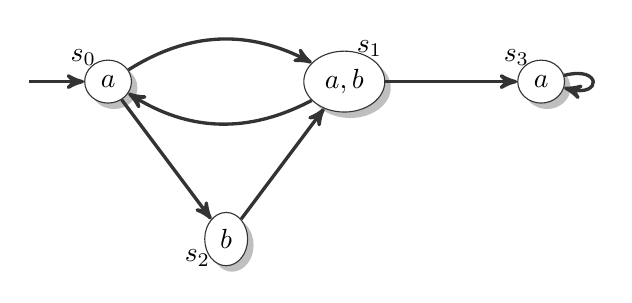
\begin{tikzpicture}
      \coordinate(init) at (-1,1);
      \node(s0) at (0,1) [oval, label={[label distance=-2mm]110:$s_0$}] {$a$};
      \node(s1) at (3,1) [oval, label={[label distance=-2mm]80:$s_1$}] {$a,b$};
      \node(s2) at (1.5,-1) [oval, label={[label distance=-2mm]190:$s_2$}] {$b$};
      \node(s3) at (5.5,1) [oval, label={[label distance=-2mm]110:$s_3$}] {$a$};
      \draw[arrow] (init) to (s0);
      \draw[arrow] (s0) to[bend left] (s1);
      \draw[arrow] (s1) to[bend left] (s0);
      \draw[arrow] (s0) to (s2);
      \draw[arrow] (s2) to (s1);
      \draw[arrow] (s1) to (s3);
      \draw[arrow] (s3) to[loop right] (s3);
    \end{tikzpicture}
  \end{center}
  \lstinputlisting[style=customConf]{../conf/book6.4.ts}
\end{frame}

\begin{frame}
  \frametitle{\acs{CTL} Model Checking}
  \begin{itemize}
  \item \alert{Verificare} se $TS\models\Phi$
    \begin{itemize}
    \item \alert{calcolare} ricorsivamente $Sat(\Phi)$
      \begin{eqnarray*}
        Sat(true)&=&S\\
        Sat(a)&=&\left\{s\in S| a\in L(s)\right\}\qquad,\forall a\in
        AP\\
        Sat(\Phi\land\Psi)&=&Sat(\Phi)\cap Sat(\Psi)\\
        Sat(\neg\Phi)&=&S\setminus Sat(\Phi)\\
        Sat(\exists\ctlNext\Phi)&=&\left\{s\in S|Post(s)\cap Sat(\Phi)\neq\varnothing\right\}\\
        Sat(\exists(\Phi\ctlUntil\Psi))&=&\text{il pi\`u piccolo }T\subseteq
        S\text{ t.c.}\\
        &&\quad Sat(\Psi)\cup\left\{s\in Sat(\Phi)|Post(s)\cap
          T\neq\varnothing\right\}\subseteq T\\
        Sat(\exists\ctlAlways\Phi)&=&\text{il pi\`u grande }T\subseteq
        S\text{ t.c.}\\
        &&\quad T\subseteq\left\{s\in Sat(\Phi)|Post(s)\cap
          T\neq\varnothing\right\}
      \end{eqnarray*}
    \item $TS\models\Phi \Leftrightarrow I\subseteq Sat(\Phi)$
    \end{itemize}
  \end{itemize}
\end{frame}

\begin{frame}[fragile]
  \frametitle{Implementazione $Sat(\cdot)$}
  \begin{pblock}
def __init__(self, ts):
    self._callDic = {
        'true':self._satTrue,
        'ap':self._satAp,
        'and':self._satAnd,
        'not':self._satNot,
        'next':self._satNext,
        'until':self._satUntil,
        'always':self._satAlways,
    }

    self._ts = ts
  \end{pblock}
  \begin{pblock}
def sat(self, phi):
    return (self._sat(phi, [s for s,a in phi.graph.nodes(data=True) if a['root'] ==True][0]))    
  \end{pblock}
  \begin{pblock}
def _sat(self, phi, nodo):
    if (phi.graph.node[nodo]['form'] in self._callDic.keys()) :
        return self._callDic[phi.graph.node[nodo]['form']](phi, nodo)    
  \end{pblock}
\end{frame}

\begin{frame}[fragile]
  \frametitle{Implementazione $Sat(\cdot)$}
  \begin{pblock}
def _satTrue(self, phi, nodo):
    return set(self._lts.graph.nodes())
  \end{pblock}

  \begin{pblock}
def _satAp(self, phi, nodo):
    retSet = set()
    for stato,att in self._lts.graph.nodes(data=True):
        if phi.graph.node[nodo]['val'] in att['att']:
           retSet.add(stato)

    return retSet    
  \end{pblock}

  \begin{pblock}
def _satAnd(self, phi, nodo):
    return self._sat(phi, phi.graph.successors(nodo)[0]).intersection(self._sat(phi, phi.graph.successors(nodo)[1]))
  \end{pblock}

  \begin{pblock}
def _satNot(self, phi, nodo):
    return set(self._lts.graph.nodes()).difference(self._sat(phi, phi.graph.successors(nodo)[0]))
  \end{pblock}
\end{frame}

\begin{frame}[fragile]
  \frametitle{Implementazione $Sat(\cdot)$}
  \begin{pblock}
def _satNext(self, phi, nodo):
    retSet = set()
    satPhi = self._sat(phi, phi.graph.successors(nodo)[0])

    for stato in self._lts.graph.nodes():
        if set(self._lts.graph.successors(stato)).intersection(satPhi): #true if not empty
            retSet.add(stato)

    return retSet
  \end{pblock}

  \begin{pblock}
def _satUntil(self, phi, nodo):
    E = self._sat(phi, phi.graph.successors(nodo)[1])
    T = E.copy()

    while E: #while not empty
        r = E.pop()
        for s in self._lts.graph.predecessors(r):
            if s in self._sat(phi, phi.graph.successors(nodo)[0]).difference(T):
                E.add(s)
                T.add(s)
    return T
  \end{pblock}
\end{frame}

\begin{frame}[fragile]
  \frametitle{Implementazione $Sat(\cdot)$}
  \begin{pblock}
def _satAlways(self, phi, nodo):
    T = self._sat(phi, phi.graph.successors(nodo)[0])
    E = set(self._lts.graph.nodes()).difference(T)
    count = dict()
    for s in T:
        count[s] = len(self._lts.graph.successors(s))

    while E:
        r = E.pop()
        for s in self._lts.graph.predecessors(r):
            if s in T:
                count[s] = count[s]-1
                if count[s] == 0:
                    T.remove(s)
                    E.add(s)

    return 
  \end{pblock}
\end{frame}

\begin{frame}[fragile]
  \frametitle{Implementazione $TS\models\Phi$}
  \begin{pblock}
def check(self, phi):
    sats = self._sat(phi, [s for s,a in phi.graph.nodes(data=True) if a['root'] ==True][0])
    initials = set([s for s,a in self._ts.graph.nodes(data=True) if a['initial'] ==True])
    return initials.issubset(sats)    
  \end{pblock}
\end{frame}

\end{document}